\documentclass[]{beamer} % die option 't' sorgt dafür, dass der content nicht automatisch auf die folie zentriert

\usepackage[english]{babel}
\usepackage[utf8]{inputenc}
\usepackage{csquotes}
\usepackage[T1]{fontenc}
\usepackage{lmodern}
\usepackage{default}
\usepackage{graphicx}
\usepackage[backend=biber,style=ieee]{biblatex}
\usepackage[acronym,shortcuts,nowarn]{glossaries}
\usepackage{enumerate}
\usepackage{wrapfig}

\graphicspath{{figures/}{imgs/}}
\bibliography{bib/db.bib}
\makeglossaries
\InputIfFileExists{abbrev/acronyms}{}{}

\usetheme{INSO}

\title{Introduction to Dining Cryptographer Networks}
\author{Jakob Gruber}
\matrnr{0203440}
\date{\today}

\setlength{\parskip}{1em}

\begin{document}

\maketitle

\begin{frame}{Outline}
	\begin{minipage}[t][10em][t]{\linewidth}
		\tableofcontents
	\end{minipage}
\end{frame}

\section{Introduction}

\begin{frame}{Introduction}
\begin{itemize}
\item Topic: anonymous group communications. Transmission of a message in a group
      of $n$ members such that an observer gains no knowledge of where the message originated.
\item Whistleblowers, resistance to repressive regimes, protecting minority rights, free speech.      
\end{itemize}

\end{frame}

\section{The \acl{DCProtocol}}

\begin{frame}{The \acl{DCProtocol}} % General properties.
Published by \citeauthor{journals/joc/Chaum88} in \citeyear{journals/joc/Chaum88}
\cite{journals/joc/Chaum88} (\citeauthor{journals/joc/Chaum88} also introduced \aclp{MixNet}).

\begin{itemize}
\item Provably strong anonymity
\item Immunity to traffic analysis
\item No reliance on trusted parties
\item Inherently limited scalability
\item Dealing with malicious group members (disruptors) is a challenge
\end{itemize}

\end{frame}

\begin{frame}{The \acl{DCProtocol}}

Demonstration of the protocol by example. Three cryptographers determine
if one of them or the NSA has paid for dinner ($n = 3, |m| = 1$ bit).

\begin{wrapfigure}{r}{0.4\textwidth}
\begin{center}
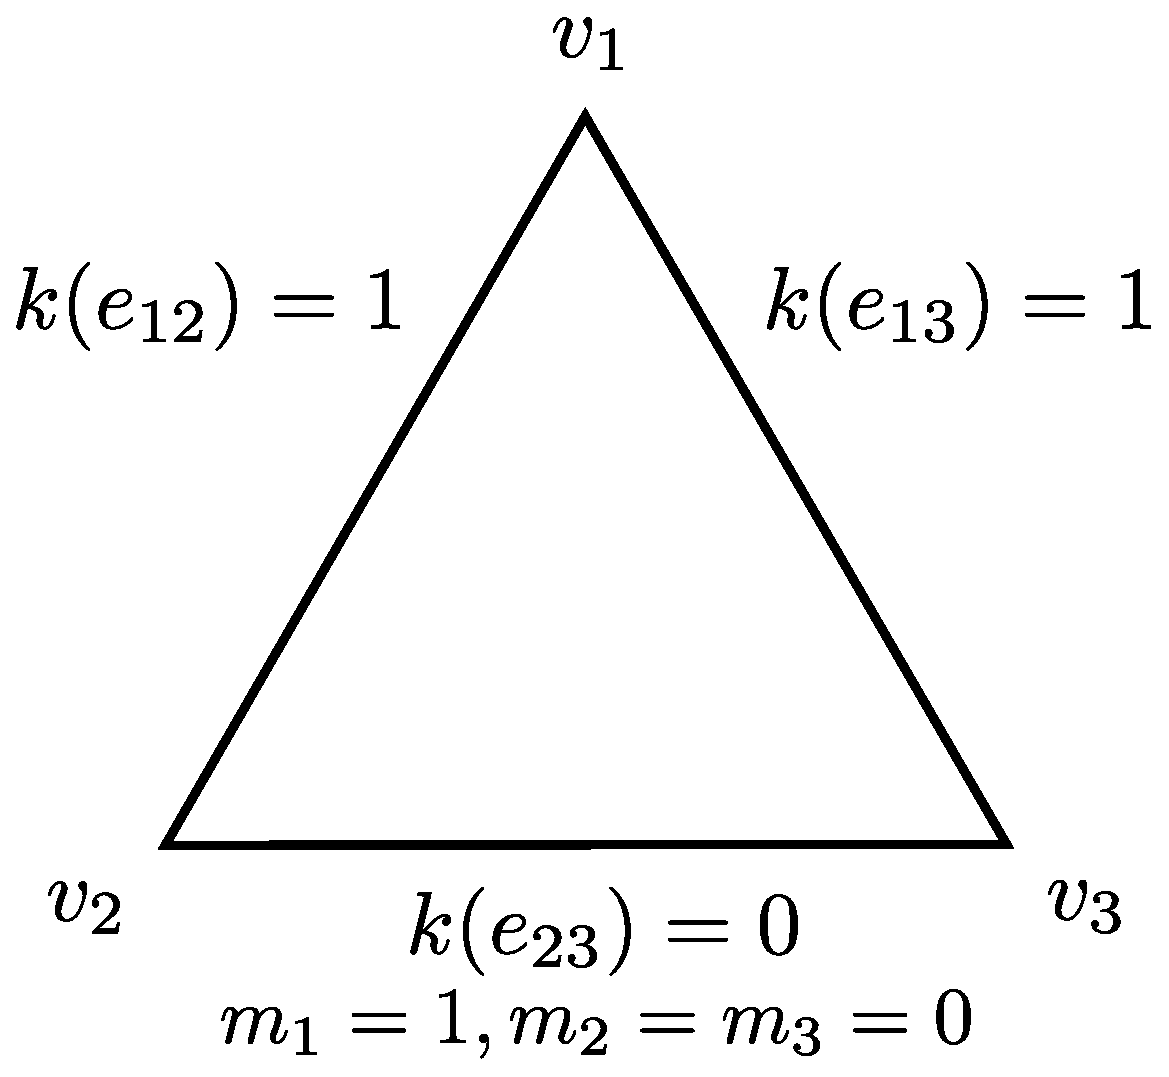
\includegraphics[width=0.38\textwidth]{keysharing_graph}
\end{center}
\end{wrapfigure}

Nodes $v_i$ represent cryptographers, edges $e_{ij}$ represent shared keys
with value $k(e_{ij}) \in \{0, 1\}$.

Keys are chosen uniformly at random and are kept secret from other nodes.
The goal is for each node $v_i$ to send a message $m_i \in \{0, 1\}$
anonymously to all other nodes with $0 \approx \text{paid}, 1 \approx \text{did not pay}$.

\end{frame}

\begin{frame}{The \acl{DCProtocol}}

\emph{Broadcast phase}: Each node forms $a(v_i)$ by XORing all of its shared keys
together with its message $m_i$, and broadcasts the result to all other members.

\begin{wrapfigure}{r}{0.4\textwidth}
\begin{center}
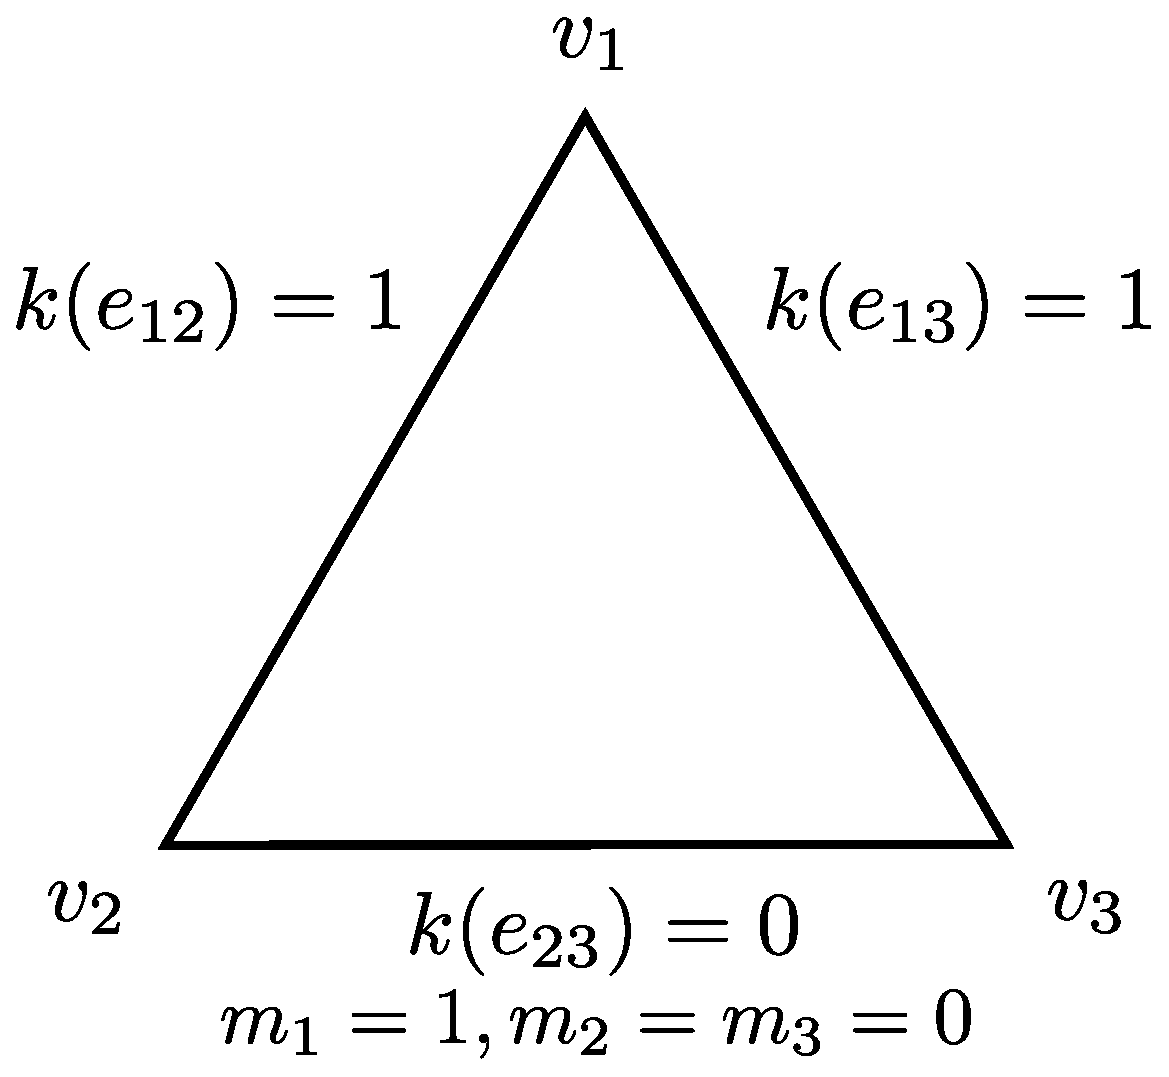
\includegraphics[width=0.38\textwidth]{keysharing_graph}
\end{center}
\end{wrapfigure}

\emph{Message reconstruction}: Finally, all $a(v_i)$ are XORed by each node to form $m'_i$.
A cryptographer paid iff $m'_i = 1$.

In this example, $\forall i: a(v_i) = 1$, and $m'_i = 1$.

\end{frame}

\begin{frame}{The \acl{DCProtocol}}

How does it work? Shared keys cancel each other out. 

\begin{align*}
m'_i &= a(v_1) \oplus a(v_2) \oplus a(v_3) \\
     &= m_1 \oplus m_2 \oplus m_3
     \oplus (k(e_{12}) \oplus k(e_{21})) \\
     & \oplus (k(e_{13}) \oplus k(e_{31})) 
     \oplus (k(e_{23}) \oplus k(e_{32})) = m_1 \oplus m_2 \oplus m_3
\end{align*}

\end{frame}

\begin{frame}{The \acl{DCProtocol}}

\begin{itemize}
\item Neither nonpaying cryptographers nor eavesdroppers gains any information as to who paid.
\item Generalize to larger groups, messages by using connected keysharing graph with $n$ nodes
      and running multiple iterations of protocol.
\item Messages may be tied to a pseudonym through signing and sent to a particular target
      through encryption.
\item Collisions: If more than one paid, the result of the protocol is invalid.
      Attackers can intentionally cause collisions to disrupt communications.
\item High message complexity of $\Omega(n^3)$.
\item Other issues: establishment of shared keys, collusion, group membership, \ldots
\end{itemize}

\end{frame}

% Maybe skip this section if presentation is too long.
\section{k-Anonymous Message Transmission}

\begin{frame}{k-Anonymous Message Transmission}

Published in \citeyear{von2003k} by \citeauthor{von2003k} \cite{von2003k}.

\begin{itemize}
\item A \ac{DCNetwork} variant
\item Tackles scalability through relaxation of security guarantees
\item Instead of full $n$-anonymity, $k$-anonymity: cannot distinguish between $k$
      senders and/or receivers
\item $O(k^2)$ messages transmitted in non-interrupted rounds, and disruptors
      are detected with high probability.
\end{itemize}

\end{frame}

\begin{frame}{k-Anonymous Message Transmission}

Three main concepts are used:

\begin{itemize}
\item Secure multiparty sums: % Elaborate here if too short
      $n$ participants with private inputs $X_i$ compute $\sum X_i$ without
      revealing any $X_i$.
\item Pedersen commitments: Publicly and irrevocably commit to a value $s$ without
      revealing $s$.
\item Zero-knowledge proofs: Prove some property without revealing additional information.
\end{itemize}

\end{frame}

\begin{frame}{k-Anonymous Message Transmission}

Rough protocol description:

\begin{itemize}
\item Form subgroups of size $M$ such that with high probability each group contains at
      least $k$ honest participants
\item The protocol is run in $2M$ iterations. Each participants chooses one slot,
      and can provide a zero-knowledge proof that at most one slot was chosen.
\item In each iteration, each participant inputs a message and target group
      $(msg_i, g_i)$. This tuple is interpreted as an integer, and a commitment
      is published.
\item The group then performs a multiparty sum to reveal message. Its authenticity can
      be verified through commitments since $C(s_1)C(s_2) = C(s_1 + s_2)$.
\end{itemize}

\end{frame}

\section{Accountable Messaging in Dissent}

\begin{frame}{Accountable Messaging in Dissent}

Published in \citeyear{journals/corr/abs-1004-3057} by \citeauthor{journals/corr/abs-1004-3057}
\cite{journals/corr/abs-1004-3057}.

\begin{itemize}
\item Misbehaving members are exposed through verifiable proofs. This property is called
      accountability.
\item Collision avoidance through a slot assignment protocol.
\item A working prototype demonstrates viability in moderate group sizes of up to 40 members.
\item Protocol consists of two subphases: Shuffle and Bulk
\end{itemize}

\end{frame}

\begin{frame}[allowframebreaks]{Accountable Messaging in Dissent}
In the \emph{shuffle protocol}, each member has: a primary encryption
(private, public) key pair $(x_i, y_i)$, a signing key pair $(u_i, v_i)$, and a message $m_i$
of fixed length $L$ common to all.

A tamper-evident log stores all sent and received messages and can be used in
case of disruption to identify the attacker.

\begin{itemize}
\item Each member $i$ generates a secondary encryption key pair $(w_i, z_i)$ and broadcasts $z_i$.
\item $m_i$ is encrypted in $2n$ layers starting with secondary encryption keys $z_n, \cdots, z_1$
      and followed by primary encryption keys $y_n, \ldots, y_1$, resulting in $C_i$ which is sent
      to member 1.
\item $\forall i:$ member $i$ receives vector $\vec{C_i}$, randomly permutes its elements,
      strips one layer of encryption, and forwards the resulting vector to $i + 1$. The final
      vector $\vec{C_n}$ is broadcast to the entire group.
\item Each member $i$ verifies that
      his encrypted $m_i$ is present, and sets the $GO_i$ flag accordingly. $GO_i$ is then broadcast
      together with a hash over all broadcast messages received or sent during the previous phases.
      If all members receive the go ahead together with the expected broadcast message log hash
      from all other members, we proceed to the final stage.
\item Each member $i$ broadcasts his secondary private key $w_i$, and finally decrypts the remaining
      layers of encryption on $\vec{C_n}$ to receive a permutation of $m_i$.
\end{itemize}

\end{frame}

\begin{frame}{Accountable Messaging in Dissent}

\begin{figure}[h!]
\centering
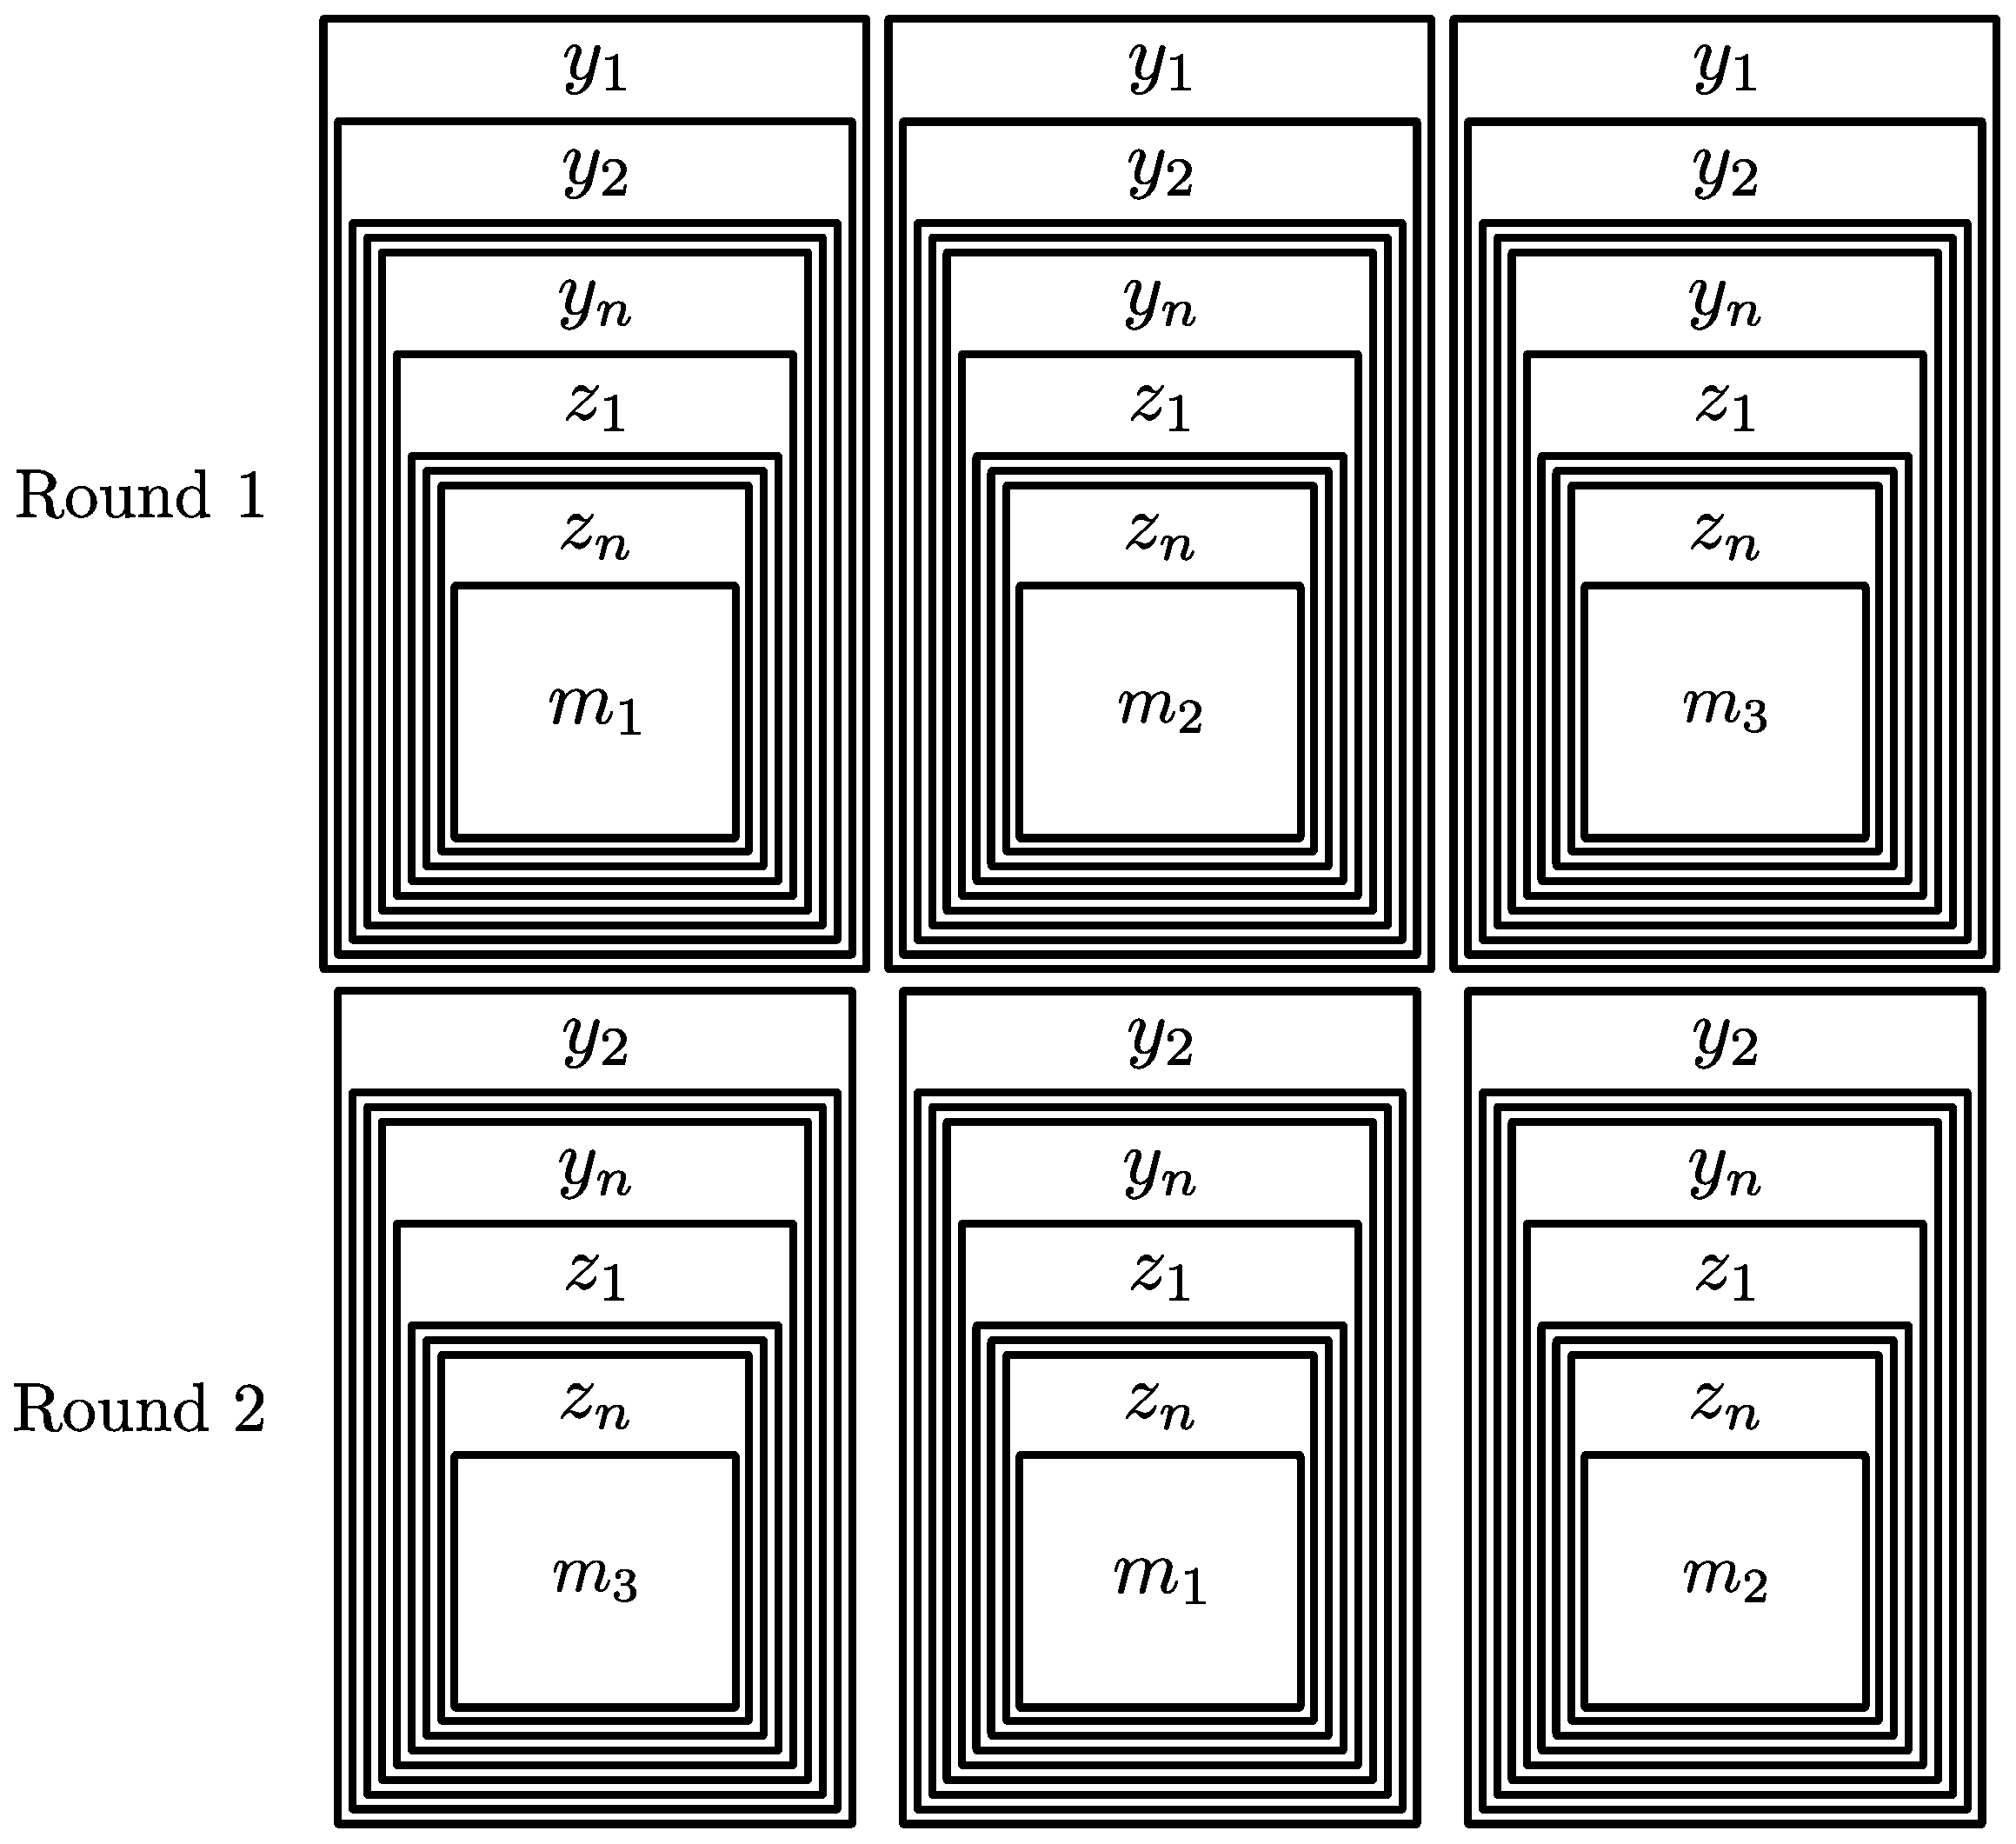
\includegraphics[width=0.75\textwidth]{dissent_shuffle}
\end{figure}

\end{frame}

\begin{frame}{Accountable Messaging in Dissent}

The \emph{bulk protocol} handles the actual transmission of messages. Again, each member has
a primary encryption and signing key pairs and a message $m_i$ of potentially varying length
$L_i$. 

\begin{itemize}
\item Essentially a modified \ac{DCProtocol}.
\item Shuffle protocol: Slot reservation, broadcast of seed values $s_{ij}$
      and message hashes $HASH(m_i)$.
\item Shared keys generated with RNG and seed value $s_{ij}$.
\item Result verifiable through hashes. On failure, faulty members can be exposed
      by replaying the log. % TODO: Study the details here.
\end{itemize}

\end{frame}

\begin{frame}{Accountable Messaging in Dissent}

\begin{itemize}
\item Faulty members are always exposed.
\item $O(n^2) + \sum L_i$ in normal case, $O(n^3) + \sum L_i$ with faulty members.
% TODO: More?
\end{itemize}

\end{frame}

\section{Related Work}

\begin{frame}{Related Work}
\begin{itemize}
\item Verdict \cite{corrigan2013proactively} is the successor to Dissent and offers
      proactively accountable messaging and an efficient hybrid mode of operation.
\item Related \ac{DCNetwork} papers \cite{waidner1989dining,juels2004dining,bos1990detection}.
\item Herbivore \cite{goel2003herbivore}, Crowds \cite{reiter1998crowds}:
      Other implementations based (in part) on \acp{DCNetwork}.
\item \acp{MixNet} \cite{journals/cacm/Chaum81}, Tor \cite{conf/uss/DingledineMS04}:
      Alternative anonymity network concept. Better scalability,
      but reliance on trusted parties and vulnerable to traffic analysis.
\end{itemize}

\end{frame}

\section{Conclusion}

\begin{frame}{Conclusion}

\begin{itemize}
\item Base \ac{DCProtocol}: Unconditional anonymity but strong assumptions,
      difficulty with disruptors, scalability issues.
\item k-Anonymous Messaging: High chance of successful transmission and
      detection of disruptors, improved scalability through relaxed requirements.
\item Dissent: Slot reservation through anonymous shuffle, accountability for
      guaranteed disruptor detection.
\end{itemize}

\end{frame}

\section{References}

\begin{frame}[allowframebreaks]{References}
\printbibliography
\end{frame}

\begin{titleframe}
\begin{center}
\alert{\Large Thank you!}
\end{center}
\end{titleframe}

\end{document}
